% Created by tikzDevice version 0.12 on 2019-02-27 16:25:49
% !TEX encoding = UTF-8 Unicode
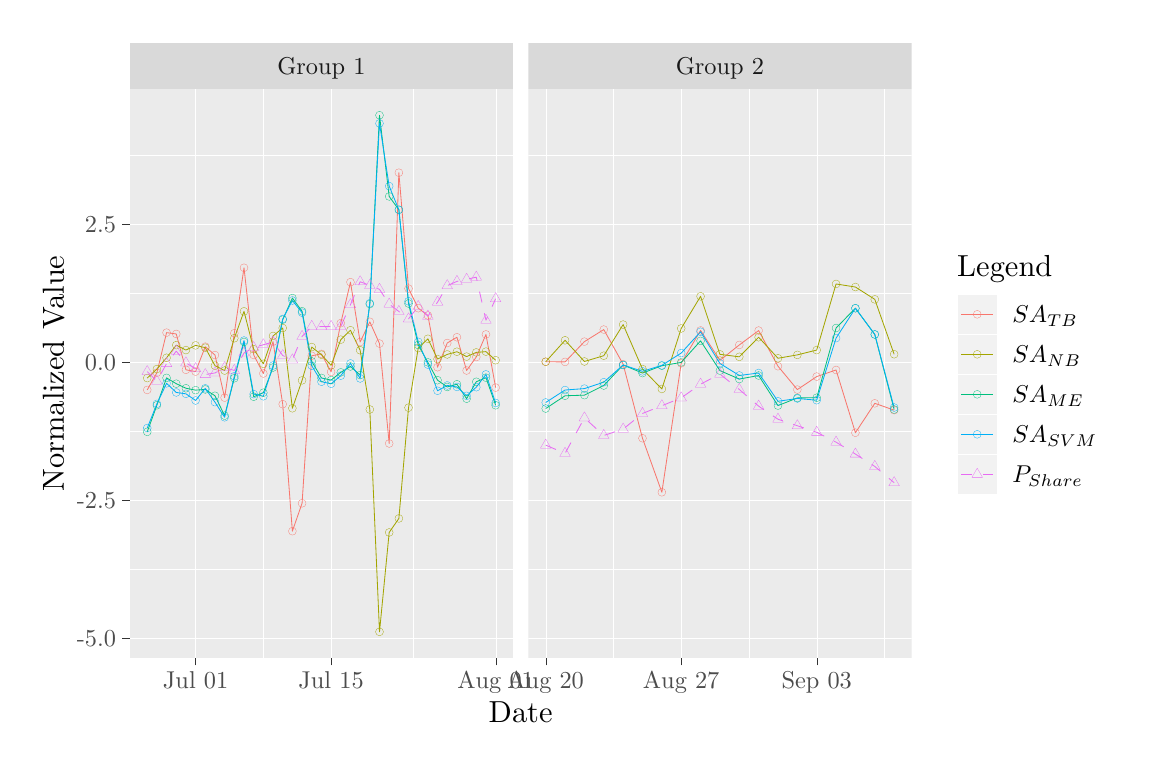
\begin{tikzpicture}[x=1pt,y=1pt]
\definecolor{fillColor}{RGB}{255,255,255}
\path[use as bounding box,fill=fillColor,fill opacity=0.00] (0,0) rectangle (397.48,258.37);
\begin{scope}
\path[clip] (  0.00,  0.00) rectangle (397.48,258.37);
\definecolor{drawColor}{RGB}{255,255,255}
\definecolor{fillColor}{RGB}{255,255,255}

\path[draw=drawColor,line width= 0.1pt,line join=round,line cap=round,fill=fillColor] (  0.00, -0.00) rectangle (397.48,258.37);
\end{scope}
\begin{scope}
\path[clip] ( 36.90, 30.73) rectangle (175.39,236.06);
\definecolor{fillColor}{gray}{0.92}

\path[fill=fillColor] ( 36.90, 30.73) rectangle (175.39,236.06);
\definecolor{drawColor}{RGB}{255,255,255}

\path[draw=drawColor,line width= 0.1pt,line join=round] ( 36.90, 62.84) --
	(175.39, 62.84);

\path[draw=drawColor,line width= 0.1pt,line join=round] ( 36.90,112.67) --
	(175.39,112.67);

\path[draw=drawColor,line width= 0.1pt,line join=round] ( 36.90,162.51) --
	(175.39,162.51);

\path[draw=drawColor,line width= 0.1pt,line join=round] ( 36.90,212.35) --
	(175.39,212.35);

\path[draw=drawColor,line width= 0.1pt,line join=round] ( 85.16, 30.73) --
	( 85.16,236.06);

\path[draw=drawColor,line width= 0.1pt,line join=round] (139.37, 30.73) --
	(139.37,236.06);

\path[draw=drawColor,line width= 0.1pt,line join=round] ( 36.90, 37.92) --
	(175.39, 37.92);

\path[draw=drawColor,line width= 0.1pt,line join=round] ( 36.90, 87.75) --
	(175.39, 87.75);

\path[draw=drawColor,line width= 0.1pt,line join=round] ( 36.90,137.59) --
	(175.39,137.59);

\path[draw=drawColor,line width= 0.1pt,line join=round] ( 36.90,187.43) --
	(175.39,187.43);

\path[draw=drawColor,line width= 0.1pt,line join=round] ( 60.68, 30.73) --
	( 60.68,236.06);

\path[draw=drawColor,line width= 0.1pt,line join=round] (109.64, 30.73) --
	(109.64,236.06);

\path[draw=drawColor,line width= 0.1pt,line join=round] (169.10, 30.73) --
	(169.10,236.06);
\definecolor{drawColor}{RGB}{248,118,109}

\path[draw=drawColor,line width= 0.3pt,line join=round] ( 43.20,127.47) --
	( 46.69,133.68) --
	( 50.19,148.17) --
	( 53.69,147.69) --
	( 57.18,134.74) --
	( 60.68,134.09) --
	( 64.18,143.10) --
	( 67.68,140.08) --
	( 71.17,124.68) --
	( 74.67,147.96) --
	( 78.17,171.61) --
	( 81.67,140.11) --
	( 85.16,133.40) --
	( 88.66,144.94) --
	( 92.16,122.32) --
	( 95.65, 76.43) --
	( 99.15, 86.51) --
	(102.65,139.81) --
	(106.15,140.49) --
	(109.64,133.99) --
	(113.14,151.60) --
	(116.64,166.41) --
	(120.14,144.78) --
	(123.63,152.08) --
	(127.13,144.22) --
	(130.63,108.12) --
	(134.13,205.96) --
	(137.62,164.09) --
	(141.12,157.01) --
	(144.62,154.37) --
	(148.11,135.67) --
	(151.61,144.42) --
	(155.11,146.51) --
	(158.61,134.49) --
	(162.10,139.36) --
	(165.60,147.53) --
	(169.10,128.31);
\definecolor{drawColor}{RGB}{163,165,0}

\path[draw=drawColor,line width= 0.3pt,line join=round] ( 43.20,131.75) --
	( 46.69,135.01) --
	( 50.19,139.09) --
	( 53.69,143.65) --
	( 57.18,141.87) --
	( 60.68,143.57) --
	( 64.18,142.73) --
	( 67.68,136.23) --
	( 71.17,134.47) --
	( 74.67,146.16) --
	( 78.17,155.87) --
	( 81.67,142.21) --
	( 85.16,136.91) --
	( 88.66,146.97) --
	( 92.16,149.85) --
	( 95.65,120.84) --
	( 99.15,130.92) --
	(102.65,142.96) --
	(106.15,140.19) --
	(109.64,136.35) --
	(113.14,145.63) --
	(116.64,149.05) --
	(120.14,141.82) --
	(123.63,120.40) --
	(127.13, 40.06) --
	(130.63, 75.97) --
	(134.13, 81.04) --
	(137.62,121.06) --
	(141.12,142.60) --
	(144.62,145.94) --
	(148.11,138.62) --
	(151.61,140.30) --
	(155.11,141.27) --
	(158.61,139.51) --
	(162.10,141.03) --
	(165.60,141.31) --
	(169.10,138.21);
\definecolor{drawColor}{RGB}{0,191,125}

\path[draw=drawColor,line width= 0.3pt,line join=round] ( 43.20,112.32) --
	( 46.69,121.94) --
	( 50.19,131.82) --
	( 53.69,129.72) --
	( 57.18,128.08) --
	( 60.68,127.39) --
	( 64.18,127.65) --
	( 67.68,125.35) --
	( 71.17,118.17) --
	( 74.67,131.71) --
	( 78.17,144.80) --
	( 81.67,125.01) --
	( 85.16,126.46) --
	( 88.66,135.57) --
	( 92.16,152.85) --
	( 95.65,160.66) --
	( 99.15,155.91) --
	(102.65,137.78) --
	(106.15,131.80) --
	(109.64,131.02) --
	(113.14,133.82) --
	(116.64,135.95) --
	(120.14,132.83) --
	(123.63,158.49) --
	(127.13,226.73) --
	(130.63,197.39) --
	(134.13,192.58) --
	(137.62,158.70) --
	(141.12,143.71) --
	(144.62,137.43) --
	(148.11,130.99) --
	(151.61,128.54) --
	(155.11,129.52) --
	(158.61,124.30) --
	(162.10,130.41) --
	(165.60,131.90) --
	(169.10,121.93);
\definecolor{drawColor}{RGB}{0,176,246}

\path[draw=drawColor,line width= 0.3pt,line join=round] ( 43.20,113.69) --
	( 46.69,122.42) --
	( 50.19,129.86) --
	( 53.69,126.56) --
	( 57.18,126.06) --
	( 60.68,123.66) --
	( 64.18,128.05) --
	( 67.68,123.05) --
	( 71.17,117.58) --
	( 74.67,132.41) --
	( 78.17,145.32) --
	( 81.67,125.96) --
	( 85.16,125.18) --
	( 88.66,136.27) --
	( 92.16,153.10) --
	( 95.65,159.79) --
	( 99.15,155.38) --
	(102.65,136.22) --
	(106.15,130.43) --
	(109.64,129.69) --
	(113.14,132.62) --
	(116.64,137.05) --
	(120.14,131.62) --
	(123.63,158.79) --
	(127.13,223.78) --
	(130.63,201.11) --
	(134.13,192.54) --
	(137.62,159.49) --
	(141.12,144.84) --
	(144.62,136.62) --
	(148.11,127.16) --
	(151.61,129.09) --
	(155.11,128.55) --
	(158.61,125.33) --
	(162.10,128.46) --
	(165.60,133.08) --
	(169.10,122.76);
\definecolor{drawColor}{RGB}{231,107,243}

\path[draw=drawColor,line width= 0.3pt,dash pattern=on 4pt off 4pt ,line join=round] ( 43.20,134.10) --
	( 46.69,130.62) --
	( 50.19,137.00) --
	( 53.69,141.47) --
	( 57.18,137.25) --
	( 60.68,135.14) --
	( 64.18,133.02) --
	( 67.68,133.60) --
	( 71.17,135.51) --
	( 74.67,134.51) --
	( 78.17,140.81) --
	( 81.67,142.79) --
	( 85.16,143.79) --
	( 88.66,144.78) --
	( 92.16,139.90) --
	( 95.65,138.32) --
	( 99.15,146.77) --
	(102.65,150.41) --
	(106.15,150.41) --
	(109.64,150.41) --
	(113.14,150.41) --
	(116.64,158.28) --
	(120.14,166.56) --
	(123.63,165.23) --
	(127.13,163.82) --
	(130.63,158.48) --
	(134.13,155.81) --
	(137.62,153.14) --
	(141.12,157.61) --
	(144.62,154.14) --
	(148.11,159.19) --
	(151.61,165.15) --
	(155.11,166.68) --
	(158.61,167.45) --
	(162.10,168.21) --
	(165.60,152.65) --
	(169.10,160.43);
\definecolor{drawColor}{RGB}{248,118,109}

\path[draw=drawColor,line width= 0.1pt,line join=round,line cap=round] ( 43.20,127.47) circle (  1.43);

\path[draw=drawColor,line width= 0.1pt,line join=round,line cap=round] ( 46.69,133.68) circle (  1.43);

\path[draw=drawColor,line width= 0.1pt,line join=round,line cap=round] ( 50.19,148.17) circle (  1.43);

\path[draw=drawColor,line width= 0.1pt,line join=round,line cap=round] ( 53.69,147.69) circle (  1.43);

\path[draw=drawColor,line width= 0.1pt,line join=round,line cap=round] ( 57.18,134.74) circle (  1.43);

\path[draw=drawColor,line width= 0.1pt,line join=round,line cap=round] ( 60.68,134.09) circle (  1.43);

\path[draw=drawColor,line width= 0.1pt,line join=round,line cap=round] ( 64.18,143.10) circle (  1.43);

\path[draw=drawColor,line width= 0.1pt,line join=round,line cap=round] ( 67.68,140.08) circle (  1.43);

\path[draw=drawColor,line width= 0.1pt,line join=round,line cap=round] ( 71.17,124.68) circle (  1.43);

\path[draw=drawColor,line width= 0.1pt,line join=round,line cap=round] ( 74.67,147.96) circle (  1.43);

\path[draw=drawColor,line width= 0.1pt,line join=round,line cap=round] ( 78.17,171.61) circle (  1.43);

\path[draw=drawColor,line width= 0.1pt,line join=round,line cap=round] ( 81.67,140.11) circle (  1.43);

\path[draw=drawColor,line width= 0.1pt,line join=round,line cap=round] ( 85.16,133.40) circle (  1.43);

\path[draw=drawColor,line width= 0.1pt,line join=round,line cap=round] ( 88.66,144.94) circle (  1.43);

\path[draw=drawColor,line width= 0.1pt,line join=round,line cap=round] ( 92.16,122.32) circle (  1.43);

\path[draw=drawColor,line width= 0.1pt,line join=round,line cap=round] ( 95.65, 76.43) circle (  1.43);

\path[draw=drawColor,line width= 0.1pt,line join=round,line cap=round] ( 99.15, 86.51) circle (  1.43);

\path[draw=drawColor,line width= 0.1pt,line join=round,line cap=round] (102.65,139.81) circle (  1.43);

\path[draw=drawColor,line width= 0.1pt,line join=round,line cap=round] (106.15,140.49) circle (  1.43);

\path[draw=drawColor,line width= 0.1pt,line join=round,line cap=round] (109.64,133.99) circle (  1.43);

\path[draw=drawColor,line width= 0.1pt,line join=round,line cap=round] (113.14,151.60) circle (  1.43);

\path[draw=drawColor,line width= 0.1pt,line join=round,line cap=round] (116.64,166.41) circle (  1.43);

\path[draw=drawColor,line width= 0.1pt,line join=round,line cap=round] (120.14,144.78) circle (  1.43);

\path[draw=drawColor,line width= 0.1pt,line join=round,line cap=round] (123.63,152.08) circle (  1.43);

\path[draw=drawColor,line width= 0.1pt,line join=round,line cap=round] (127.13,144.22) circle (  1.43);

\path[draw=drawColor,line width= 0.1pt,line join=round,line cap=round] (130.63,108.12) circle (  1.43);

\path[draw=drawColor,line width= 0.1pt,line join=round,line cap=round] (134.13,205.96) circle (  1.43);

\path[draw=drawColor,line width= 0.1pt,line join=round,line cap=round] (137.62,164.09) circle (  1.43);

\path[draw=drawColor,line width= 0.1pt,line join=round,line cap=round] (141.12,157.01) circle (  1.43);

\path[draw=drawColor,line width= 0.1pt,line join=round,line cap=round] (144.62,154.37) circle (  1.43);

\path[draw=drawColor,line width= 0.1pt,line join=round,line cap=round] (148.11,135.67) circle (  1.43);

\path[draw=drawColor,line width= 0.1pt,line join=round,line cap=round] (151.61,144.42) circle (  1.43);

\path[draw=drawColor,line width= 0.1pt,line join=round,line cap=round] (155.11,146.51) circle (  1.43);

\path[draw=drawColor,line width= 0.1pt,line join=round,line cap=round] (158.61,134.49) circle (  1.43);

\path[draw=drawColor,line width= 0.1pt,line join=round,line cap=round] (162.10,139.36) circle (  1.43);

\path[draw=drawColor,line width= 0.1pt,line join=round,line cap=round] (165.60,147.53) circle (  1.43);

\path[draw=drawColor,line width= 0.1pt,line join=round,line cap=round] (169.10,128.31) circle (  1.43);
\definecolor{drawColor}{RGB}{163,165,0}

\path[draw=drawColor,line width= 0.1pt,line join=round,line cap=round] ( 43.20,131.75) circle (  1.43);

\path[draw=drawColor,line width= 0.1pt,line join=round,line cap=round] ( 46.69,135.01) circle (  1.43);

\path[draw=drawColor,line width= 0.1pt,line join=round,line cap=round] ( 50.19,139.09) circle (  1.43);

\path[draw=drawColor,line width= 0.1pt,line join=round,line cap=round] ( 53.69,143.65) circle (  1.43);

\path[draw=drawColor,line width= 0.1pt,line join=round,line cap=round] ( 57.18,141.87) circle (  1.43);

\path[draw=drawColor,line width= 0.1pt,line join=round,line cap=round] ( 60.68,143.57) circle (  1.43);

\path[draw=drawColor,line width= 0.1pt,line join=round,line cap=round] ( 64.18,142.73) circle (  1.43);

\path[draw=drawColor,line width= 0.1pt,line join=round,line cap=round] ( 67.68,136.23) circle (  1.43);

\path[draw=drawColor,line width= 0.1pt,line join=round,line cap=round] ( 71.17,134.47) circle (  1.43);

\path[draw=drawColor,line width= 0.1pt,line join=round,line cap=round] ( 74.67,146.16) circle (  1.43);

\path[draw=drawColor,line width= 0.1pt,line join=round,line cap=round] ( 78.17,155.87) circle (  1.43);

\path[draw=drawColor,line width= 0.1pt,line join=round,line cap=round] ( 81.67,142.21) circle (  1.43);

\path[draw=drawColor,line width= 0.1pt,line join=round,line cap=round] ( 85.16,136.91) circle (  1.43);

\path[draw=drawColor,line width= 0.1pt,line join=round,line cap=round] ( 88.66,146.97) circle (  1.43);

\path[draw=drawColor,line width= 0.1pt,line join=round,line cap=round] ( 92.16,149.85) circle (  1.43);

\path[draw=drawColor,line width= 0.1pt,line join=round,line cap=round] ( 95.65,120.84) circle (  1.43);

\path[draw=drawColor,line width= 0.1pt,line join=round,line cap=round] ( 99.15,130.92) circle (  1.43);

\path[draw=drawColor,line width= 0.1pt,line join=round,line cap=round] (102.65,142.96) circle (  1.43);

\path[draw=drawColor,line width= 0.1pt,line join=round,line cap=round] (106.15,140.19) circle (  1.43);

\path[draw=drawColor,line width= 0.1pt,line join=round,line cap=round] (109.64,136.35) circle (  1.43);

\path[draw=drawColor,line width= 0.1pt,line join=round,line cap=round] (113.14,145.63) circle (  1.43);

\path[draw=drawColor,line width= 0.1pt,line join=round,line cap=round] (116.64,149.05) circle (  1.43);

\path[draw=drawColor,line width= 0.1pt,line join=round,line cap=round] (120.14,141.82) circle (  1.43);

\path[draw=drawColor,line width= 0.1pt,line join=round,line cap=round] (123.63,120.40) circle (  1.43);

\path[draw=drawColor,line width= 0.1pt,line join=round,line cap=round] (127.13, 40.06) circle (  1.43);

\path[draw=drawColor,line width= 0.1pt,line join=round,line cap=round] (130.63, 75.97) circle (  1.43);

\path[draw=drawColor,line width= 0.1pt,line join=round,line cap=round] (134.13, 81.04) circle (  1.43);

\path[draw=drawColor,line width= 0.1pt,line join=round,line cap=round] (137.62,121.06) circle (  1.43);

\path[draw=drawColor,line width= 0.1pt,line join=round,line cap=round] (141.12,142.60) circle (  1.43);

\path[draw=drawColor,line width= 0.1pt,line join=round,line cap=round] (144.62,145.94) circle (  1.43);

\path[draw=drawColor,line width= 0.1pt,line join=round,line cap=round] (148.11,138.62) circle (  1.43);

\path[draw=drawColor,line width= 0.1pt,line join=round,line cap=round] (151.61,140.30) circle (  1.43);

\path[draw=drawColor,line width= 0.1pt,line join=round,line cap=round] (155.11,141.27) circle (  1.43);

\path[draw=drawColor,line width= 0.1pt,line join=round,line cap=round] (158.61,139.51) circle (  1.43);

\path[draw=drawColor,line width= 0.1pt,line join=round,line cap=round] (162.10,141.03) circle (  1.43);

\path[draw=drawColor,line width= 0.1pt,line join=round,line cap=round] (165.60,141.31) circle (  1.43);

\path[draw=drawColor,line width= 0.1pt,line join=round,line cap=round] (169.10,138.21) circle (  1.43);
\definecolor{drawColor}{RGB}{0,191,125}

\path[draw=drawColor,line width= 0.1pt,line join=round,line cap=round] ( 43.20,112.32) circle (  1.43);

\path[draw=drawColor,line width= 0.1pt,line join=round,line cap=round] ( 46.69,121.94) circle (  1.43);

\path[draw=drawColor,line width= 0.1pt,line join=round,line cap=round] ( 50.19,131.82) circle (  1.43);

\path[draw=drawColor,line width= 0.1pt,line join=round,line cap=round] ( 53.69,129.72) circle (  1.43);

\path[draw=drawColor,line width= 0.1pt,line join=round,line cap=round] ( 57.18,128.08) circle (  1.43);

\path[draw=drawColor,line width= 0.1pt,line join=round,line cap=round] ( 60.68,127.39) circle (  1.43);

\path[draw=drawColor,line width= 0.1pt,line join=round,line cap=round] ( 64.18,127.65) circle (  1.43);

\path[draw=drawColor,line width= 0.1pt,line join=round,line cap=round] ( 67.68,125.35) circle (  1.43);

\path[draw=drawColor,line width= 0.1pt,line join=round,line cap=round] ( 71.17,118.17) circle (  1.43);

\path[draw=drawColor,line width= 0.1pt,line join=round,line cap=round] ( 74.67,131.71) circle (  1.43);

\path[draw=drawColor,line width= 0.1pt,line join=round,line cap=round] ( 78.17,144.80) circle (  1.43);

\path[draw=drawColor,line width= 0.1pt,line join=round,line cap=round] ( 81.67,125.01) circle (  1.43);

\path[draw=drawColor,line width= 0.1pt,line join=round,line cap=round] ( 85.16,126.46) circle (  1.43);

\path[draw=drawColor,line width= 0.1pt,line join=round,line cap=round] ( 88.66,135.57) circle (  1.43);

\path[draw=drawColor,line width= 0.1pt,line join=round,line cap=round] ( 92.16,152.85) circle (  1.43);

\path[draw=drawColor,line width= 0.1pt,line join=round,line cap=round] ( 95.65,160.66) circle (  1.43);

\path[draw=drawColor,line width= 0.1pt,line join=round,line cap=round] ( 99.15,155.91) circle (  1.43);

\path[draw=drawColor,line width= 0.1pt,line join=round,line cap=round] (102.65,137.78) circle (  1.43);

\path[draw=drawColor,line width= 0.1pt,line join=round,line cap=round] (106.15,131.80) circle (  1.43);

\path[draw=drawColor,line width= 0.1pt,line join=round,line cap=round] (109.64,131.02) circle (  1.43);

\path[draw=drawColor,line width= 0.1pt,line join=round,line cap=round] (113.14,133.82) circle (  1.43);

\path[draw=drawColor,line width= 0.1pt,line join=round,line cap=round] (116.64,135.95) circle (  1.43);

\path[draw=drawColor,line width= 0.1pt,line join=round,line cap=round] (120.14,132.83) circle (  1.43);

\path[draw=drawColor,line width= 0.1pt,line join=round,line cap=round] (123.63,158.49) circle (  1.43);

\path[draw=drawColor,line width= 0.1pt,line join=round,line cap=round] (127.13,226.73) circle (  1.43);

\path[draw=drawColor,line width= 0.1pt,line join=round,line cap=round] (130.63,197.39) circle (  1.43);

\path[draw=drawColor,line width= 0.1pt,line join=round,line cap=round] (134.13,192.58) circle (  1.43);

\path[draw=drawColor,line width= 0.1pt,line join=round,line cap=round] (137.62,158.70) circle (  1.43);

\path[draw=drawColor,line width= 0.1pt,line join=round,line cap=round] (141.12,143.71) circle (  1.43);

\path[draw=drawColor,line width= 0.1pt,line join=round,line cap=round] (144.62,137.43) circle (  1.43);

\path[draw=drawColor,line width= 0.1pt,line join=round,line cap=round] (148.11,130.99) circle (  1.43);

\path[draw=drawColor,line width= 0.1pt,line join=round,line cap=round] (151.61,128.54) circle (  1.43);

\path[draw=drawColor,line width= 0.1pt,line join=round,line cap=round] (155.11,129.52) circle (  1.43);

\path[draw=drawColor,line width= 0.1pt,line join=round,line cap=round] (158.61,124.30) circle (  1.43);

\path[draw=drawColor,line width= 0.1pt,line join=round,line cap=round] (162.10,130.41) circle (  1.43);

\path[draw=drawColor,line width= 0.1pt,line join=round,line cap=round] (165.60,131.90) circle (  1.43);

\path[draw=drawColor,line width= 0.1pt,line join=round,line cap=round] (169.10,121.93) circle (  1.43);
\definecolor{drawColor}{RGB}{0,176,246}

\path[draw=drawColor,line width= 0.1pt,line join=round,line cap=round] ( 43.20,113.69) circle (  1.43);

\path[draw=drawColor,line width= 0.1pt,line join=round,line cap=round] ( 46.69,122.42) circle (  1.43);

\path[draw=drawColor,line width= 0.1pt,line join=round,line cap=round] ( 50.19,129.86) circle (  1.43);

\path[draw=drawColor,line width= 0.1pt,line join=round,line cap=round] ( 53.69,126.56) circle (  1.43);

\path[draw=drawColor,line width= 0.1pt,line join=round,line cap=round] ( 57.18,126.06) circle (  1.43);

\path[draw=drawColor,line width= 0.1pt,line join=round,line cap=round] ( 60.68,123.66) circle (  1.43);

\path[draw=drawColor,line width= 0.1pt,line join=round,line cap=round] ( 64.18,128.05) circle (  1.43);

\path[draw=drawColor,line width= 0.1pt,line join=round,line cap=round] ( 67.68,123.05) circle (  1.43);

\path[draw=drawColor,line width= 0.1pt,line join=round,line cap=round] ( 71.17,117.58) circle (  1.43);

\path[draw=drawColor,line width= 0.1pt,line join=round,line cap=round] ( 74.67,132.41) circle (  1.43);

\path[draw=drawColor,line width= 0.1pt,line join=round,line cap=round] ( 78.17,145.32) circle (  1.43);

\path[draw=drawColor,line width= 0.1pt,line join=round,line cap=round] ( 81.67,125.96) circle (  1.43);

\path[draw=drawColor,line width= 0.1pt,line join=round,line cap=round] ( 85.16,125.18) circle (  1.43);

\path[draw=drawColor,line width= 0.1pt,line join=round,line cap=round] ( 88.66,136.27) circle (  1.43);

\path[draw=drawColor,line width= 0.1pt,line join=round,line cap=round] ( 92.16,153.10) circle (  1.43);

\path[draw=drawColor,line width= 0.1pt,line join=round,line cap=round] ( 95.65,159.79) circle (  1.43);

\path[draw=drawColor,line width= 0.1pt,line join=round,line cap=round] ( 99.15,155.38) circle (  1.43);

\path[draw=drawColor,line width= 0.1pt,line join=round,line cap=round] (102.65,136.22) circle (  1.43);

\path[draw=drawColor,line width= 0.1pt,line join=round,line cap=round] (106.15,130.43) circle (  1.43);

\path[draw=drawColor,line width= 0.1pt,line join=round,line cap=round] (109.64,129.69) circle (  1.43);

\path[draw=drawColor,line width= 0.1pt,line join=round,line cap=round] (113.14,132.62) circle (  1.43);

\path[draw=drawColor,line width= 0.1pt,line join=round,line cap=round] (116.64,137.05) circle (  1.43);

\path[draw=drawColor,line width= 0.1pt,line join=round,line cap=round] (120.14,131.62) circle (  1.43);

\path[draw=drawColor,line width= 0.1pt,line join=round,line cap=round] (123.63,158.79) circle (  1.43);

\path[draw=drawColor,line width= 0.1pt,line join=round,line cap=round] (127.13,223.78) circle (  1.43);

\path[draw=drawColor,line width= 0.1pt,line join=round,line cap=round] (130.63,201.11) circle (  1.43);

\path[draw=drawColor,line width= 0.1pt,line join=round,line cap=round] (134.13,192.54) circle (  1.43);

\path[draw=drawColor,line width= 0.1pt,line join=round,line cap=round] (137.62,159.49) circle (  1.43);

\path[draw=drawColor,line width= 0.1pt,line join=round,line cap=round] (141.12,144.84) circle (  1.43);

\path[draw=drawColor,line width= 0.1pt,line join=round,line cap=round] (144.62,136.62) circle (  1.43);

\path[draw=drawColor,line width= 0.1pt,line join=round,line cap=round] (148.11,127.16) circle (  1.43);

\path[draw=drawColor,line width= 0.1pt,line join=round,line cap=round] (151.61,129.09) circle (  1.43);

\path[draw=drawColor,line width= 0.1pt,line join=round,line cap=round] (155.11,128.55) circle (  1.43);

\path[draw=drawColor,line width= 0.1pt,line join=round,line cap=round] (158.61,125.33) circle (  1.43);

\path[draw=drawColor,line width= 0.1pt,line join=round,line cap=round] (162.10,128.46) circle (  1.43);

\path[draw=drawColor,line width= 0.1pt,line join=round,line cap=round] (165.60,133.08) circle (  1.43);

\path[draw=drawColor,line width= 0.1pt,line join=round,line cap=round] (169.10,122.76) circle (  1.43);
\definecolor{drawColor}{RGB}{231,107,243}

\path[draw=drawColor,line width= 0.1pt,line join=round,line cap=round] ( 43.20,136.32) --
	( 45.12,132.99) --
	( 41.27,132.99) --
	( 43.20,136.32);

\path[draw=drawColor,line width= 0.1pt,line join=round,line cap=round] ( 46.69,132.84) --
	( 48.61,129.51) --
	( 44.77,129.51) --
	( 46.69,132.84);

\path[draw=drawColor,line width= 0.1pt,line join=round,line cap=round] ( 50.19,139.22) --
	( 52.11,135.89) --
	( 48.27,135.89) --
	( 50.19,139.22);

\path[draw=drawColor,line width= 0.1pt,line join=round,line cap=round] ( 53.69,143.69) --
	( 55.61,140.36) --
	( 51.77,140.36) --
	( 53.69,143.69);

\path[draw=drawColor,line width= 0.1pt,line join=round,line cap=round] ( 57.18,139.47) --
	( 59.11,136.14) --
	( 55.26,136.14) --
	( 57.18,139.47);

\path[draw=drawColor,line width= 0.1pt,line join=round,line cap=round] ( 60.68,137.35) --
	( 62.60,134.03) --
	( 58.76,134.03) --
	( 60.68,137.35);

\path[draw=drawColor,line width= 0.1pt,line join=round,line cap=round] ( 64.18,135.24) --
	( 66.10,131.91) --
	( 62.26,131.91) --
	( 64.18,135.24);

\path[draw=drawColor,line width= 0.1pt,line join=round,line cap=round] ( 67.68,135.82) --
	( 69.60,132.49) --
	( 65.75,132.49) --
	( 67.68,135.82);

\path[draw=drawColor,line width= 0.1pt,line join=round,line cap=round] ( 71.17,137.73) --
	( 73.09,134.40) --
	( 69.25,134.40) --
	( 71.17,137.73);

\path[draw=drawColor,line width= 0.1pt,line join=round,line cap=round] ( 74.67,136.73) --
	( 76.59,133.41) --
	( 72.75,133.41) --
	( 74.67,136.73);

\path[draw=drawColor,line width= 0.1pt,line join=round,line cap=round] ( 78.17,143.03) --
	( 80.09,139.70) --
	( 76.25,139.70) --
	( 78.17,143.03);

\path[draw=drawColor,line width= 0.1pt,line join=round,line cap=round] ( 81.67,145.01) --
	( 83.59,141.68) --
	( 79.74,141.68) --
	( 81.67,145.01);

\path[draw=drawColor,line width= 0.1pt,line join=round,line cap=round] ( 85.16,146.01) --
	( 87.08,142.68) --
	( 83.24,142.68) --
	( 85.16,146.01);

\path[draw=drawColor,line width= 0.1pt,line join=round,line cap=round] ( 88.66,147.00) --
	( 90.58,143.67) --
	( 86.74,143.67) --
	( 88.66,147.00);

\path[draw=drawColor,line width= 0.1pt,line join=round,line cap=round] ( 92.16,142.11) --
	( 94.08,138.79) --
	( 90.24,138.79) --
	( 92.16,142.11);

\path[draw=drawColor,line width= 0.1pt,line join=round,line cap=round] ( 95.65,140.54) --
	( 97.58,137.21) --
	( 93.73,137.21) --
	( 95.65,140.54);

\path[draw=drawColor,line width= 0.1pt,line join=round,line cap=round] ( 99.15,148.99) --
	(101.07,145.66) --
	( 97.23,145.66) --
	( 99.15,148.99);

\path[draw=drawColor,line width= 0.1pt,line join=round,line cap=round] (102.65,152.63) --
	(104.57,149.30) --
	(100.73,149.30) --
	(102.65,152.63);

\path[draw=drawColor,line width= 0.1pt,line join=round,line cap=round] (106.15,152.63) --
	(108.07,149.30) --
	(104.23,149.30) --
	(106.15,152.63);

\path[draw=drawColor,line width= 0.1pt,line join=round,line cap=round] (109.64,152.63) --
	(111.57,149.30) --
	(107.72,149.30) --
	(109.64,152.63);

\path[draw=drawColor,line width= 0.1pt,line join=round,line cap=round] (113.14,152.63) --
	(115.06,149.30) --
	(111.22,149.30) --
	(113.14,152.63);

\path[draw=drawColor,line width= 0.1pt,line join=round,line cap=round] (116.64,160.49) --
	(118.56,157.17) --
	(114.72,157.17) --
	(116.64,160.49);

\path[draw=drawColor,line width= 0.1pt,line join=round,line cap=round] (120.14,168.77) --
	(122.06,165.45) --
	(118.21,165.45) --
	(120.14,168.77);

\path[draw=drawColor,line width= 0.1pt,line join=round,line cap=round] (123.63,167.45) --
	(125.55,164.12) --
	(121.71,164.12) --
	(123.63,167.45);

\path[draw=drawColor,line width= 0.1pt,line join=round,line cap=round] (127.13,166.04) --
	(129.05,162.71) --
	(125.21,162.71) --
	(127.13,166.04);

\path[draw=drawColor,line width= 0.1pt,line join=round,line cap=round] (130.63,160.70) --
	(132.55,157.37) --
	(128.71,157.37) --
	(130.63,160.70);

\path[draw=drawColor,line width= 0.1pt,line join=round,line cap=round] (134.13,158.03) --
	(136.05,154.70) --
	(132.20,154.70) --
	(134.13,158.03);

\path[draw=drawColor,line width= 0.1pt,line join=round,line cap=round] (137.62,155.36) --
	(139.54,152.03) --
	(135.70,152.03) --
	(137.62,155.36);

\path[draw=drawColor,line width= 0.1pt,line join=round,line cap=round] (141.12,159.83) --
	(143.04,156.50) --
	(139.20,156.50) --
	(141.12,159.83);

\path[draw=drawColor,line width= 0.1pt,line join=round,line cap=round] (144.62,156.36) --
	(146.54,153.03) --
	(142.70,153.03) --
	(144.62,156.36);

\path[draw=drawColor,line width= 0.1pt,line join=round,line cap=round] (148.11,161.41) --
	(150.04,158.08) --
	(146.19,158.08) --
	(148.11,161.41);

\path[draw=drawColor,line width= 0.1pt,line join=round,line cap=round] (151.61,167.37) --
	(153.53,164.04) --
	(149.69,164.04) --
	(151.61,167.37);

\path[draw=drawColor,line width= 0.1pt,line join=round,line cap=round] (155.11,168.90) --
	(157.03,165.57) --
	(153.19,165.57) --
	(155.11,168.90);

\path[draw=drawColor,line width= 0.1pt,line join=round,line cap=round] (158.61,169.66) --
	(160.53,166.34) --
	(156.69,166.34) --
	(158.61,169.66);

\path[draw=drawColor,line width= 0.1pt,line join=round,line cap=round] (162.10,170.43) --
	(164.03,167.10) --
	(160.18,167.10) --
	(162.10,170.43);

\path[draw=drawColor,line width= 0.1pt,line join=round,line cap=round] (165.60,154.86) --
	(167.52,151.54) --
	(163.68,151.54) --
	(165.60,154.86);

\path[draw=drawColor,line width= 0.1pt,line join=round,line cap=round] (169.10,162.65) --
	(171.02,159.32) --
	(167.18,159.32) --
	(169.10,162.65);
\end{scope}
\begin{scope}
\path[clip] (180.89, 30.73) rectangle (319.39,236.06);
\definecolor{fillColor}{gray}{0.92}

\path[fill=fillColor] (180.89, 30.73) rectangle (319.39,236.06);
\definecolor{drawColor}{RGB}{255,255,255}

\path[draw=drawColor,line width= 0.1pt,line join=round] (180.89, 62.84) --
	(319.39, 62.84);

\path[draw=drawColor,line width= 0.1pt,line join=round] (180.89,112.67) --
	(319.39,112.67);

\path[draw=drawColor,line width= 0.1pt,line join=round] (180.89,162.51) --
	(319.39,162.51);

\path[draw=drawColor,line width= 0.1pt,line join=round] (180.89,212.35) --
	(319.39,212.35);

\path[draw=drawColor,line width= 0.1pt,line join=round] (211.67, 30.73) --
	(211.67,236.06);

\path[draw=drawColor,line width= 0.1pt,line join=round] (260.63, 30.73) --
	(260.63,236.06);

\path[draw=drawColor,line width= 0.1pt,line join=round] (309.59, 30.73) --
	(309.59,236.06);

\path[draw=drawColor,line width= 0.1pt,line join=round] (180.89, 37.92) --
	(319.39, 37.92);

\path[draw=drawColor,line width= 0.1pt,line join=round] (180.89, 87.75) --
	(319.39, 87.75);

\path[draw=drawColor,line width= 0.1pt,line join=round] (180.89,137.59) --
	(319.39,137.59);

\path[draw=drawColor,line width= 0.1pt,line join=round] (180.89,187.43) --
	(319.39,187.43);

\path[draw=drawColor,line width= 0.1pt,line join=round] (187.19, 30.73) --
	(187.19,236.06);

\path[draw=drawColor,line width= 0.1pt,line join=round] (236.15, 30.73) --
	(236.15,236.06);

\path[draw=drawColor,line width= 0.1pt,line join=round] (285.11, 30.73) --
	(285.11,236.06);
\definecolor{drawColor}{RGB}{248,118,109}

\path[draw=drawColor,line width= 0.3pt,line join=round] (187.19,137.65) --
	(194.18,137.59) --
	(201.18,144.92) --
	(208.17,149.28) --
	(215.17,136.76) --
	(222.16,110.01) --
	(229.16, 90.49) --
	(236.15,137.09) --
	(243.15,148.97) --
	(250.14,138.15) --
	(257.14,143.72) --
	(264.13,148.92) --
	(271.12,136.04) --
	(278.12,127.59) --
	(285.11,132.29) --
	(292.11,134.68) --
	(299.10,112.01) --
	(306.10,122.63) --
	(313.09,120.16);
\definecolor{drawColor}{RGB}{163,165,0}

\path[draw=drawColor,line width= 0.3pt,line join=round] (187.19,137.65) --
	(194.18,145.41) --
	(201.18,137.75) --
	(208.17,139.84) --
	(215.17,151.08) --
	(222.16,135.02) --
	(229.16,127.82) --
	(236.15,149.69) --
	(243.15,161.29) --
	(250.14,140.33) --
	(257.14,139.43) --
	(264.13,146.51) --
	(271.12,138.91) --
	(278.12,140.13) --
	(285.11,141.87) --
	(292.11,165.76) --
	(299.10,164.65) --
	(306.10,160.20) --
	(313.09,140.37);
\definecolor{drawColor}{RGB}{0,191,125}

\path[draw=drawColor,line width= 0.3pt,line join=round] (187.19,120.75) --
	(194.18,125.36) --
	(201.18,125.58) --
	(208.17,129.06) --
	(215.17,136.48) --
	(222.16,133.56) --
	(229.16,136.21) --
	(236.15,137.41) --
	(243.15,145.20) --
	(250.14,134.44) --
	(257.14,131.41) --
	(264.13,132.67) --
	(271.12,121.81) --
	(278.12,124.58) --
	(285.11,124.65) --
	(292.11,149.84) --
	(299.10,157.00) --
	(306.10,147.50) --
	(313.09,120.39);
\definecolor{drawColor}{RGB}{0,176,246}

\path[draw=drawColor,line width= 0.3pt,line join=round] (187.19,122.93) --
	(194.18,127.43) --
	(201.18,127.95) --
	(208.17,130.26) --
	(215.17,136.49) --
	(222.16,134.19) --
	(229.16,136.35) --
	(236.15,140.79) --
	(243.15,148.49) --
	(250.14,137.03) --
	(257.14,132.69) --
	(264.13,133.58) --
	(271.12,123.36) --
	(278.12,124.38) --
	(285.11,123.76) --
	(292.11,146.20) --
	(299.10,156.98) --
	(306.10,147.54) --
	(313.09,121.10);
\definecolor{drawColor}{RGB}{231,107,243}

\path[draw=drawColor,line width= 0.3pt,dash pattern=on 4pt off 4pt ,line join=round] (187.19,107.52) --
	(194.18,104.54) --
	(201.18,117.38) --
	(208.17,111.00) --
	(215.17,113.32) --
	(222.16,118.95) --
	(229.16,121.76) --
	(236.15,124.58) --
	(243.15,129.55) --
	(250.14,133.19) --
	(257.14,127.64) --
	(264.13,121.60) --
	(271.12,116.88) --
	(278.12,114.52) --
	(285.11,112.16) --
	(292.11,108.60) --
	(299.10,104.29) --
	(306.10, 99.82) --
	(313.09, 93.95);
\definecolor{drawColor}{RGB}{248,118,109}

\path[draw=drawColor,line width= 0.1pt,line join=round,line cap=round] (187.19,137.65) circle (  1.43);

\path[draw=drawColor,line width= 0.1pt,line join=round,line cap=round] (194.18,137.59) circle (  1.43);

\path[draw=drawColor,line width= 0.1pt,line join=round,line cap=round] (201.18,144.92) circle (  1.43);

\path[draw=drawColor,line width= 0.1pt,line join=round,line cap=round] (208.17,149.28) circle (  1.43);

\path[draw=drawColor,line width= 0.1pt,line join=round,line cap=round] (215.17,136.76) circle (  1.43);

\path[draw=drawColor,line width= 0.1pt,line join=round,line cap=round] (222.16,110.01) circle (  1.43);

\path[draw=drawColor,line width= 0.1pt,line join=round,line cap=round] (229.16, 90.49) circle (  1.43);

\path[draw=drawColor,line width= 0.1pt,line join=round,line cap=round] (236.15,137.09) circle (  1.43);

\path[draw=drawColor,line width= 0.1pt,line join=round,line cap=round] (243.15,148.97) circle (  1.43);

\path[draw=drawColor,line width= 0.1pt,line join=round,line cap=round] (250.14,138.15) circle (  1.43);

\path[draw=drawColor,line width= 0.1pt,line join=round,line cap=round] (257.14,143.72) circle (  1.43);

\path[draw=drawColor,line width= 0.1pt,line join=round,line cap=round] (264.13,148.92) circle (  1.43);

\path[draw=drawColor,line width= 0.1pt,line join=round,line cap=round] (271.12,136.04) circle (  1.43);

\path[draw=drawColor,line width= 0.1pt,line join=round,line cap=round] (278.12,127.59) circle (  1.43);

\path[draw=drawColor,line width= 0.1pt,line join=round,line cap=round] (285.11,132.29) circle (  1.43);

\path[draw=drawColor,line width= 0.1pt,line join=round,line cap=round] (292.11,134.68) circle (  1.43);

\path[draw=drawColor,line width= 0.1pt,line join=round,line cap=round] (299.10,112.01) circle (  1.43);

\path[draw=drawColor,line width= 0.1pt,line join=round,line cap=round] (306.10,122.63) circle (  1.43);

\path[draw=drawColor,line width= 0.1pt,line join=round,line cap=round] (313.09,120.16) circle (  1.43);
\definecolor{drawColor}{RGB}{163,165,0}

\path[draw=drawColor,line width= 0.1pt,line join=round,line cap=round] (187.19,137.65) circle (  1.43);

\path[draw=drawColor,line width= 0.1pt,line join=round,line cap=round] (194.18,145.41) circle (  1.43);

\path[draw=drawColor,line width= 0.1pt,line join=round,line cap=round] (201.18,137.75) circle (  1.43);

\path[draw=drawColor,line width= 0.1pt,line join=round,line cap=round] (208.17,139.84) circle (  1.43);

\path[draw=drawColor,line width= 0.1pt,line join=round,line cap=round] (215.17,151.08) circle (  1.43);

\path[draw=drawColor,line width= 0.1pt,line join=round,line cap=round] (222.16,135.02) circle (  1.43);

\path[draw=drawColor,line width= 0.1pt,line join=round,line cap=round] (229.16,127.82) circle (  1.43);

\path[draw=drawColor,line width= 0.1pt,line join=round,line cap=round] (236.15,149.69) circle (  1.43);

\path[draw=drawColor,line width= 0.1pt,line join=round,line cap=round] (243.15,161.29) circle (  1.43);

\path[draw=drawColor,line width= 0.1pt,line join=round,line cap=round] (250.14,140.33) circle (  1.43);

\path[draw=drawColor,line width= 0.1pt,line join=round,line cap=round] (257.14,139.43) circle (  1.43);

\path[draw=drawColor,line width= 0.1pt,line join=round,line cap=round] (264.13,146.51) circle (  1.43);

\path[draw=drawColor,line width= 0.1pt,line join=round,line cap=round] (271.12,138.91) circle (  1.43);

\path[draw=drawColor,line width= 0.1pt,line join=round,line cap=round] (278.12,140.13) circle (  1.43);

\path[draw=drawColor,line width= 0.1pt,line join=round,line cap=round] (285.11,141.87) circle (  1.43);

\path[draw=drawColor,line width= 0.1pt,line join=round,line cap=round] (292.11,165.76) circle (  1.43);

\path[draw=drawColor,line width= 0.1pt,line join=round,line cap=round] (299.10,164.65) circle (  1.43);

\path[draw=drawColor,line width= 0.1pt,line join=round,line cap=round] (306.10,160.20) circle (  1.43);

\path[draw=drawColor,line width= 0.1pt,line join=round,line cap=round] (313.09,140.37) circle (  1.43);
\definecolor{drawColor}{RGB}{0,191,125}

\path[draw=drawColor,line width= 0.1pt,line join=round,line cap=round] (187.19,120.75) circle (  1.43);

\path[draw=drawColor,line width= 0.1pt,line join=round,line cap=round] (194.18,125.36) circle (  1.43);

\path[draw=drawColor,line width= 0.1pt,line join=round,line cap=round] (201.18,125.58) circle (  1.43);

\path[draw=drawColor,line width= 0.1pt,line join=round,line cap=round] (208.17,129.06) circle (  1.43);

\path[draw=drawColor,line width= 0.1pt,line join=round,line cap=round] (215.17,136.48) circle (  1.43);

\path[draw=drawColor,line width= 0.1pt,line join=round,line cap=round] (222.16,133.56) circle (  1.43);

\path[draw=drawColor,line width= 0.1pt,line join=round,line cap=round] (229.16,136.21) circle (  1.43);

\path[draw=drawColor,line width= 0.1pt,line join=round,line cap=round] (236.15,137.41) circle (  1.43);

\path[draw=drawColor,line width= 0.1pt,line join=round,line cap=round] (243.15,145.20) circle (  1.43);

\path[draw=drawColor,line width= 0.1pt,line join=round,line cap=round] (250.14,134.44) circle (  1.43);

\path[draw=drawColor,line width= 0.1pt,line join=round,line cap=round] (257.14,131.41) circle (  1.43);

\path[draw=drawColor,line width= 0.1pt,line join=round,line cap=round] (264.13,132.67) circle (  1.43);

\path[draw=drawColor,line width= 0.1pt,line join=round,line cap=round] (271.12,121.81) circle (  1.43);

\path[draw=drawColor,line width= 0.1pt,line join=round,line cap=round] (278.12,124.58) circle (  1.43);

\path[draw=drawColor,line width= 0.1pt,line join=round,line cap=round] (285.11,124.65) circle (  1.43);

\path[draw=drawColor,line width= 0.1pt,line join=round,line cap=round] (292.11,149.84) circle (  1.43);

\path[draw=drawColor,line width= 0.1pt,line join=round,line cap=round] (299.10,157.00) circle (  1.43);

\path[draw=drawColor,line width= 0.1pt,line join=round,line cap=round] (306.10,147.50) circle (  1.43);

\path[draw=drawColor,line width= 0.1pt,line join=round,line cap=round] (313.09,120.39) circle (  1.43);
\definecolor{drawColor}{RGB}{0,176,246}

\path[draw=drawColor,line width= 0.1pt,line join=round,line cap=round] (187.19,122.93) circle (  1.43);

\path[draw=drawColor,line width= 0.1pt,line join=round,line cap=round] (194.18,127.43) circle (  1.43);

\path[draw=drawColor,line width= 0.1pt,line join=round,line cap=round] (201.18,127.95) circle (  1.43);

\path[draw=drawColor,line width= 0.1pt,line join=round,line cap=round] (208.17,130.26) circle (  1.43);

\path[draw=drawColor,line width= 0.1pt,line join=round,line cap=round] (215.17,136.49) circle (  1.43);

\path[draw=drawColor,line width= 0.1pt,line join=round,line cap=round] (222.16,134.19) circle (  1.43);

\path[draw=drawColor,line width= 0.1pt,line join=round,line cap=round] (229.16,136.35) circle (  1.43);

\path[draw=drawColor,line width= 0.1pt,line join=round,line cap=round] (236.15,140.79) circle (  1.43);

\path[draw=drawColor,line width= 0.1pt,line join=round,line cap=round] (243.15,148.49) circle (  1.43);

\path[draw=drawColor,line width= 0.1pt,line join=round,line cap=round] (250.14,137.03) circle (  1.43);

\path[draw=drawColor,line width= 0.1pt,line join=round,line cap=round] (257.14,132.69) circle (  1.43);

\path[draw=drawColor,line width= 0.1pt,line join=round,line cap=round] (264.13,133.58) circle (  1.43);

\path[draw=drawColor,line width= 0.1pt,line join=round,line cap=round] (271.12,123.36) circle (  1.43);

\path[draw=drawColor,line width= 0.1pt,line join=round,line cap=round] (278.12,124.38) circle (  1.43);

\path[draw=drawColor,line width= 0.1pt,line join=round,line cap=round] (285.11,123.76) circle (  1.43);

\path[draw=drawColor,line width= 0.1pt,line join=round,line cap=round] (292.11,146.20) circle (  1.43);

\path[draw=drawColor,line width= 0.1pt,line join=round,line cap=round] (299.10,156.98) circle (  1.43);

\path[draw=drawColor,line width= 0.1pt,line join=round,line cap=round] (306.10,147.54) circle (  1.43);

\path[draw=drawColor,line width= 0.1pt,line join=round,line cap=round] (313.09,121.10) circle (  1.43);
\definecolor{drawColor}{RGB}{231,107,243}

\path[draw=drawColor,line width= 0.1pt,line join=round,line cap=round] (187.19,109.74) --
	(189.11,106.41) --
	(185.27,106.41) --
	(187.19,109.74);

\path[draw=drawColor,line width= 0.1pt,line join=round,line cap=round] (194.18,106.76) --
	(196.10,103.43) --
	(192.26,103.43) --
	(194.18,106.76);

\path[draw=drawColor,line width= 0.1pt,line join=round,line cap=round] (201.18,119.59) --
	(203.10,116.27) --
	(199.26,116.27) --
	(201.18,119.59);

\path[draw=drawColor,line width= 0.1pt,line join=round,line cap=round] (208.17,113.22) --
	(210.09,109.89) --
	(206.25,109.89) --
	(208.17,113.22);

\path[draw=drawColor,line width= 0.1pt,line join=round,line cap=round] (215.17,115.54) --
	(217.09,112.21) --
	(213.25,112.21) --
	(215.17,115.54);

\path[draw=drawColor,line width= 0.1pt,line join=round,line cap=round] (222.16,121.17) --
	(224.08,117.84) --
	(220.24,117.84) --
	(222.16,121.17);

\path[draw=drawColor,line width= 0.1pt,line join=round,line cap=round] (229.16,123.98) --
	(231.08,120.65) --
	(227.24,120.65) --
	(229.16,123.98);

\path[draw=drawColor,line width= 0.1pt,line join=round,line cap=round] (236.15,126.80) --
	(238.07,123.47) --
	(234.23,123.47) --
	(236.15,126.80);

\path[draw=drawColor,line width= 0.1pt,line join=round,line cap=round] (243.15,131.77) --
	(245.07,128.44) --
	(241.22,128.44) --
	(243.15,131.77);

\path[draw=drawColor,line width= 0.1pt,line join=round,line cap=round] (250.14,135.41) --
	(252.06,132.08) --
	(248.22,132.08) --
	(250.14,135.41);

\path[draw=drawColor,line width= 0.1pt,line join=round,line cap=round] (257.14,129.86) --
	(259.06,126.53) --
	(255.21,126.53) --
	(257.14,129.86);

\path[draw=drawColor,line width= 0.1pt,line join=round,line cap=round] (264.13,123.82) --
	(266.05,120.49) --
	(262.21,120.49) --
	(264.13,123.82);

\path[draw=drawColor,line width= 0.1pt,line join=round,line cap=round] (271.12,119.10) --
	(273.05,115.77) --
	(269.20,115.77) --
	(271.12,119.10);

\path[draw=drawColor,line width= 0.1pt,line join=round,line cap=round] (278.12,116.74) --
	(280.04,113.41) --
	(276.20,113.41) --
	(278.12,116.74);

\path[draw=drawColor,line width= 0.1pt,line join=round,line cap=round] (285.11,114.38) --
	(287.03,111.05) --
	(283.19,111.05) --
	(285.11,114.38);

\path[draw=drawColor,line width= 0.1pt,line join=round,line cap=round] (292.11,110.82) --
	(294.03,107.49) --
	(290.19,107.49) --
	(292.11,110.82);

\path[draw=drawColor,line width= 0.1pt,line join=round,line cap=round] (299.10,106.51) --
	(301.02,103.19) --
	(297.18,103.19) --
	(299.10,106.51);

\path[draw=drawColor,line width= 0.1pt,line join=round,line cap=round] (306.10,102.04) --
	(308.02, 98.71) --
	(304.18, 98.71) --
	(306.10,102.04);

\path[draw=drawColor,line width= 0.1pt,line join=round,line cap=round] (313.09, 96.16) --
	(315.01, 92.84) --
	(311.17, 92.84) --
	(313.09, 96.16);
\end{scope}
\begin{scope}
\path[clip] ( 36.90,236.06) rectangle (175.39,252.87);
\definecolor{fillColor}{gray}{0.85}

\path[fill=fillColor] ( 36.90,236.06) rectangle (175.39,252.87);
\definecolor{drawColor}{gray}{0.10}

\node[text=drawColor,anchor=base,inner sep=0pt, outer sep=0pt, scale=  0.88] at (106.15,241.43) {Group 1};
\end{scope}
\begin{scope}
\path[clip] (180.89,236.06) rectangle (319.39,252.87);
\definecolor{fillColor}{gray}{0.85}

\path[fill=fillColor] (180.89,236.06) rectangle (319.39,252.87);
\definecolor{drawColor}{gray}{0.10}

\node[text=drawColor,anchor=base,inner sep=0pt, outer sep=0pt, scale=  0.88] at (250.14,241.43) {Group 2};
\end{scope}
\begin{scope}
\path[clip] (  0.00,  0.00) rectangle (397.48,258.37);
\definecolor{drawColor}{gray}{0.20}

\path[draw=drawColor,line width= 0.1pt,line join=round] ( 60.68, 27.98) --
	( 60.68, 30.73);

\path[draw=drawColor,line width= 0.1pt,line join=round] (109.64, 27.98) --
	(109.64, 30.73);

\path[draw=drawColor,line width= 0.1pt,line join=round] (169.10, 27.98) --
	(169.10, 30.73);
\end{scope}
\begin{scope}
\path[clip] (  0.00,  0.00) rectangle (397.48,258.37);
\definecolor{drawColor}{gray}{0.30}

\node[text=drawColor,anchor=base,inner sep=0pt, outer sep=0pt, scale=  0.88] at ( 60.68, 19.72) {Jul 01};

\node[text=drawColor,anchor=base,inner sep=0pt, outer sep=0pt, scale=  0.88] at (109.64, 19.72) {Jul 15};

\node[text=drawColor,anchor=base,inner sep=0pt, outer sep=0pt, scale=  0.88] at (169.10, 19.72) {Aug 01};
\end{scope}
\begin{scope}
\path[clip] (  0.00,  0.00) rectangle (397.48,258.37);
\definecolor{drawColor}{gray}{0.20}

\path[draw=drawColor,line width= 0.1pt,line join=round] (187.19, 27.98) --
	(187.19, 30.73);

\path[draw=drawColor,line width= 0.1pt,line join=round] (236.15, 27.98) --
	(236.15, 30.73);

\path[draw=drawColor,line width= 0.1pt,line join=round] (285.11, 27.98) --
	(285.11, 30.73);
\end{scope}
\begin{scope}
\path[clip] (  0.00,  0.00) rectangle (397.48,258.37);
\definecolor{drawColor}{gray}{0.30}

\node[text=drawColor,anchor=base,inner sep=0pt, outer sep=0pt, scale=  0.88] at (187.19, 19.72) {Aug 20};

\node[text=drawColor,anchor=base,inner sep=0pt, outer sep=0pt, scale=  0.88] at (236.15, 19.72) {Aug 27};

\node[text=drawColor,anchor=base,inner sep=0pt, outer sep=0pt, scale=  0.88] at (285.11, 19.72) {Sep 03};
\end{scope}
\begin{scope}
\path[clip] (  0.00,  0.00) rectangle (397.48,258.37);
\definecolor{drawColor}{gray}{0.30}

\node[text=drawColor,anchor=base east,inner sep=0pt, outer sep=0pt, scale=  0.88] at ( 31.95, 34.89) {-5.0};

\node[text=drawColor,anchor=base east,inner sep=0pt, outer sep=0pt, scale=  0.88] at ( 31.95, 84.72) {-2.5};

\node[text=drawColor,anchor=base east,inner sep=0pt, outer sep=0pt, scale=  0.88] at ( 31.95,134.56) {0.0};

\node[text=drawColor,anchor=base east,inner sep=0pt, outer sep=0pt, scale=  0.88] at ( 31.95,184.40) {2.5};
\end{scope}
\begin{scope}
\path[clip] (  0.00,  0.00) rectangle (397.48,258.37);
\definecolor{drawColor}{gray}{0.20}

\path[draw=drawColor,line width= 0.1pt,line join=round] ( 34.15, 37.92) --
	( 36.90, 37.92);

\path[draw=drawColor,line width= 0.1pt,line join=round] ( 34.15, 87.75) --
	( 36.90, 87.75);

\path[draw=drawColor,line width= 0.1pt,line join=round] ( 34.15,137.59) --
	( 36.90,137.59);

\path[draw=drawColor,line width= 0.1pt,line join=round] ( 34.15,187.43) --
	( 36.90,187.43);
\end{scope}
\begin{scope}
\path[clip] (  0.00,  0.00) rectangle (397.48,258.37);
\definecolor{drawColor}{RGB}{0,0,0}

\node[text=drawColor,anchor=base,inner sep=0pt, outer sep=0pt, scale=  1.10] at (178.14,  7.44) {Date};
\end{scope}
\begin{scope}
\path[clip] (  0.00,  0.00) rectangle (397.48,258.37);
\definecolor{drawColor}{RGB}{0,0,0}

\node[text=drawColor,rotate= 90.00,anchor=base,inner sep=0pt, outer sep=0pt, scale=  1.10] at ( 13.08,133.39) {Normalized Value};
\end{scope}
\begin{scope}
\path[clip] (  0.00,  0.00) rectangle (397.48,258.37);
\definecolor{fillColor}{RGB}{255,255,255}

\path[fill=fillColor] (330.39, 84.25) rectangle (391.98,182.54);
\end{scope}
\begin{scope}
\path[clip] (  0.00,  0.00) rectangle (397.48,258.37);
\definecolor{drawColor}{RGB}{0,0,0}

\node[text=drawColor,anchor=base west,inner sep=0pt, outer sep=0pt, scale=  1.10] at (335.89,168.49) {Legend};
\end{scope}
\begin{scope}
\path[clip] (  0.00,  0.00) rectangle (397.48,258.37);
\definecolor{drawColor}{RGB}{255,255,255}
\definecolor{fillColor}{gray}{0.95}

\path[draw=drawColor,line width= 0.1pt,line join=round,line cap=round,fill=fillColor] (335.89,147.56) rectangle (350.34,162.02);
\end{scope}
\begin{scope}
\path[clip] (  0.00,  0.00) rectangle (397.48,258.37);
\definecolor{drawColor}{RGB}{248,118,109}

\path[draw=drawColor,line width= 0.3pt,line join=round] (337.33,154.79) -- (348.90,154.79);
\end{scope}
\begin{scope}
\path[clip] (  0.00,  0.00) rectangle (397.48,258.37);
\definecolor{drawColor}{RGB}{248,118,109}

\path[draw=drawColor,line width= 0.1pt,line join=round,line cap=round] (343.11,154.79) circle (  1.43);
\end{scope}
\begin{scope}
\path[clip] (  0.00,  0.00) rectangle (397.48,258.37);
\definecolor{drawColor}{RGB}{255,255,255}
\definecolor{fillColor}{gray}{0.95}

\path[draw=drawColor,line width= 0.1pt,line join=round,line cap=round,fill=fillColor] (335.89,133.11) rectangle (350.34,147.56);
\end{scope}
\begin{scope}
\path[clip] (  0.00,  0.00) rectangle (397.48,258.37);
\definecolor{drawColor}{RGB}{163,165,0}

\path[draw=drawColor,line width= 0.3pt,line join=round] (337.33,140.34) -- (348.90,140.34);
\end{scope}
\begin{scope}
\path[clip] (  0.00,  0.00) rectangle (397.48,258.37);
\definecolor{drawColor}{RGB}{163,165,0}

\path[draw=drawColor,line width= 0.1pt,line join=round,line cap=round] (343.11,140.34) circle (  1.43);
\end{scope}
\begin{scope}
\path[clip] (  0.00,  0.00) rectangle (397.48,258.37);
\definecolor{drawColor}{RGB}{255,255,255}
\definecolor{fillColor}{gray}{0.95}

\path[draw=drawColor,line width= 0.1pt,line join=round,line cap=round,fill=fillColor] (335.89,118.66) rectangle (350.34,133.11);
\end{scope}
\begin{scope}
\path[clip] (  0.00,  0.00) rectangle (397.48,258.37);
\definecolor{drawColor}{RGB}{0,191,125}

\path[draw=drawColor,line width= 0.3pt,line join=round] (337.33,125.88) -- (348.90,125.88);
\end{scope}
\begin{scope}
\path[clip] (  0.00,  0.00) rectangle (397.48,258.37);
\definecolor{drawColor}{RGB}{0,191,125}

\path[draw=drawColor,line width= 0.1pt,line join=round,line cap=round] (343.11,125.88) circle (  1.43);
\end{scope}
\begin{scope}
\path[clip] (  0.00,  0.00) rectangle (397.48,258.37);
\definecolor{drawColor}{RGB}{255,255,255}
\definecolor{fillColor}{gray}{0.95}

\path[draw=drawColor,line width= 0.1pt,line join=round,line cap=round,fill=fillColor] (335.89,104.20) rectangle (350.34,118.66);
\end{scope}
\begin{scope}
\path[clip] (  0.00,  0.00) rectangle (397.48,258.37);
\definecolor{drawColor}{RGB}{0,176,246}

\path[draw=drawColor,line width= 0.3pt,line join=round] (337.33,111.43) -- (348.90,111.43);
\end{scope}
\begin{scope}
\path[clip] (  0.00,  0.00) rectangle (397.48,258.37);
\definecolor{drawColor}{RGB}{0,176,246}

\path[draw=drawColor,line width= 0.1pt,line join=round,line cap=round] (343.11,111.43) circle (  1.43);
\end{scope}
\begin{scope}
\path[clip] (  0.00,  0.00) rectangle (397.48,258.37);
\definecolor{drawColor}{RGB}{255,255,255}
\definecolor{fillColor}{gray}{0.95}

\path[draw=drawColor,line width= 0.1pt,line join=round,line cap=round,fill=fillColor] (335.89, 89.75) rectangle (350.34,104.20);
\end{scope}
\begin{scope}
\path[clip] (  0.00,  0.00) rectangle (397.48,258.37);
\definecolor{drawColor}{RGB}{231,107,243}

\path[draw=drawColor,line width= 0.3pt,dash pattern=on 4pt off 4pt ,line join=round] (337.33, 96.97) -- (348.90, 96.97);
\end{scope}
\begin{scope}
\path[clip] (  0.00,  0.00) rectangle (397.48,258.37);
\definecolor{drawColor}{RGB}{231,107,243}

\path[draw=drawColor,line width= 0.1pt,line join=round,line cap=round] (343.11, 99.19) --
	(345.04, 95.87) --
	(341.19, 95.87) --
	(343.11, 99.19);
\end{scope}
\begin{scope}
\path[clip] (  0.00,  0.00) rectangle (397.48,258.37);
\definecolor{drawColor}{RGB}{0,0,0}

\node[text=drawColor,anchor=base west,inner sep=0pt, outer sep=0pt, scale=  0.88] at (355.84,151.76) {$SA_{TB}$};
\end{scope}
\begin{scope}
\path[clip] (  0.00,  0.00) rectangle (397.48,258.37);
\definecolor{drawColor}{RGB}{0,0,0}

\node[text=drawColor,anchor=base west,inner sep=0pt, outer sep=0pt, scale=  0.88] at (355.84,137.31) {$SA_{NB}$};
\end{scope}
\begin{scope}
\path[clip] (  0.00,  0.00) rectangle (397.48,258.37);
\definecolor{drawColor}{RGB}{0,0,0}

\node[text=drawColor,anchor=base west,inner sep=0pt, outer sep=0pt, scale=  0.88] at (355.84,122.85) {$SA_{ME}$};
\end{scope}
\begin{scope}
\path[clip] (  0.00,  0.00) rectangle (397.48,258.37);
\definecolor{drawColor}{RGB}{0,0,0}

\node[text=drawColor,anchor=base west,inner sep=0pt, outer sep=0pt, scale=  0.88] at (355.84,108.40) {$SA_{SVM}$};
\end{scope}
\begin{scope}
\path[clip] (  0.00,  0.00) rectangle (397.48,258.37);
\definecolor{drawColor}{RGB}{0,0,0}

\node[text=drawColor,anchor=base west,inner sep=0pt, outer sep=0pt, scale=  0.88] at (355.84, 93.94) {$P_{Share}$};
\end{scope}
\end{tikzpicture}
